\documentclass[conference]{IEEEtran}

\usepackage[utf8]{inputenc}
\usepackage[T1]{fontenc}
\usepackage{amsmath}
\usepackage{graphicx}
\usepackage{booktabs}
\usepackage{xcolor}
\usepackage{tikz}
\usetikzlibrary{arrows.meta,positioning,shapes.geometric}
\usepackage{url}

% Inline TODO marker -- remove before submission
\newcommand{\todo}[1]{\textcolor{red}{[TODO: #1]}}

\begin{document}

\title{CS471 Project Proposal: PolyRack-Beyond Hotness\\
\large Tiered Memory Management Beyond Hotness}

\author{
\IEEEauthorblockN{Mayeul Besnard}
\IEEEauthorblockA{EPFL\\
Lausanne, Switzerland\\
mayeul.besnard@epfl.ch}
\and
\IEEEauthorblockN{Sergio Boffi}
\IEEEauthorblockA{EPFL\\
Lausanne, Switzerland\\
sergio.boffi@epfl.ch}
}

\maketitle

\begin{abstract}
Tiered memory systems combine a fast tier (local DRAM) with a larger but slower
tier (e.g., CXL-attached memory) and typically decide data placement based on
access frequency (``hotness''). Liu et al.~\cite{liu2025tiered} argue that hot
data is not necessarily performance-critical, because memory-level parallelism
(MLP) can hide most of the slow-tier latency of some accesses but not of
others. They introduce the Amortized Offcore Latency (AOL) metric and build two
mechanisms on top of it: SOAR, an AOL-guided first-placement policy, and ALTO,
an AOL-based filter for page migrations. In this project we will reproduce the
main claims of the paper (hotness is a poor proxy of performance, AOL is a
better predictor of slowdown, SOAR and ALTO outperform state-of-the-art tiering
systems) on a traditional server and, if time permits, evaluate whether these
techniques also improve memory management on the PolyRack disaggregated rack
architecture~\cite{polyrack}.
\end{abstract}

% =====================================================================
\section{Introduction and Problem Statement}
\label{sec:problem}

\subsection{Why is the problem important?}
Server performance can be measured in many different ways, but the most common and relevant remains the number of instructions executed per cycle: $\text{Perf} \propto \text{IPC} = 1/\text{CPI}$.
Whenever the CPU requests data from memory, an LLC (Last-Level Cache) miss may occur, meaning that the requested piece of data is not available in any of the cache levels.
When this happens, the CPU might wait many cycles to get an answer from the main memory (stall cycles), and therefore performance starts degrading.
Memory-intensive datacenter workloads keep growing in footprint, and provisioning all of
their memory in DRAM is expensive. 
Tiered memory architectures add a
cheaper, higher-capacity slow tier (CXL memory, remote NUMA node) next to the
fast DRAM tier. Since the new tier is slower (2--3$\times$ slower than DRAM), the way data is distributed across tiers
determines how many memory stalls the application suffers.

\subsection{What is involved in the problem?}
The problem involves:
\begin{itemize}
    \item The two memory tiers and their latencies $T_{\text{DRAM}}$ and $T_{\text{CXL}}$
    \item The access pattern of each object
    \item Hot and cold objects/pages
    \item The initial placement policy
    \item The page migration policy
\end{itemize} 
 
A simple first-order model makes the dependencies explicit. Let $\alpha$ be the
fraction of memory accesses served by DRAM. The average memory latency is
\begin{equation}
T_{\text{total}} = \alpha\,T_{\text{DRAM}} + (1-\alpha)\,T_{\text{CXL}}.
\end{equation}
Let $\beta_{\text{DRAM,hot}}$ ($\beta_{\text{CXL,hot}}$) be the fraction of
DRAM (CXL) accesses that target hot data. Splitting the accesses to each tier
into hot and cold data gives
\begin{align}
T_{\text{total}} ={}& \underbrace{\alpha\,\beta_{\text{DRAM,hot}}T_{\text{DRAM}}}_{\text{accesses to hot data in DRAM}}
 + \underbrace{\alpha\,(1-\beta_{\text{DRAM,hot}})T_{\text{DRAM}}}_{\text{accesses to cold data in DRAM}} \nonumber\\
 &+ \underbrace{(1-\alpha)\,\beta_{\text{CXL,hot}}T_{\text{CXL}}}_{\text{accesses to hot data in CXL}}
 + \underbrace{(1-\alpha)(1-\beta_{\text{CXL,hot}})T_{\text{CXL}}}_{\text{accesses to cold data in CXL}}.
\end{align}
SOTA tiering systems put hot data into DRAM, and following this model, this means that we decrease $(1-\alpha)\,\beta_{\text{CXL,hot}}T_{\text{CXL}}$ to increase $\alpha\,\beta_{\text{DRAM,hot}}T_{\text{DRAM}}$.
Since we know that CXL accesses are more costly in terms of latency, this might look like an optimal solution, but the next section shows why this tiering system doesn't always help lower $T_{\text{total}}$.

\subsection{What causes the problem?}
First, we need to point out that slow-tier accesses and page migrations are expensive in terms of latency (each migration can take several $\mu$s).
To reduce the slowdown, we need to find a way to decide whether a page should migrate or whether an object should be placed in the fast or the slow tier.
Having an effective initial placement algorithm allows us to have fewer page migrations, hence reducing the total slowdown.
As we have seen, SOTA uses hotness as a metric to make tiering decisions, but hotness ignores memory-level parallelism (MLP).
In out-of-order (OoO) cores, memory requests can be overlapped (when possible), so the effective cost of an access is the latency of that access divided by the number of concurrent accesses.
This breaks the assumption of the model above, where every access pays the
full latency of its tier.

Let us consider two different data structures of the same size that need to be repeatedly scanned: an array and a linked list.
When scanning an array, we already know the address of each element of the array, but in a linked list, we need to read element x to be able to reach element x+1.
Suppose we perform this scan on a tiered memory system with an OoO processor: the accesses to the array can be parallelized ($MLP \ge 1$), while the accesses to the linked list must be serialized ($MLP = 1$).
Let us suppose that hotness is measured over a fixed period of time. We can now imagine that the array has been accessed many times, making it hotter, so it gets placed in the fast tier.
This decision might help us reach the array faster, but it drastically increases the time needed to access the linked list.
Swapping the positions leads us to a lower total slowdown.


Hotness therefore measures how \emph{often} data is accessed, but not how
much each access \emph{costs}: it is an unfaithful proxy of performance.

\subsection{Does prior work solve the problem?}
No. SOTA tiering systems such as TPP, Nomad, Linux NUMA Balancing Tiering
(NBT) and Colloid all rely on hotness. On the paper's microbenchmark (one
sequential, high-MLP ``hot'' thread and one pointer-chasing, low-MLP ``cold''
thread), they underperform even a naive \emph{Cold-on-DRAM} placement, and
fall behind first-touch allocation without migrations (NoTier) by
12--14\%~\cite[Fig.~1]{liu2025tiered}. On real workloads such as
\texttt{bc-urand} (GAPBS betweenness centrality on a uniform random graph),
they can be up to 217\% slower than NoTier~\cite[Fig.~4]{liu2025tiered}.

\subsection{Problem definition, scope and success criteria}
\textbf{Problem.} \emph{Reduce the slowdown of memory-intensive workloads on
tiered memory systems, by reproducing and validating the AOL-based approach
of on our hardware and, if time permits, on PolyRack.}

\textbf{Scope.}
\begin{itemize}
  \item \emph{Infrastructure:} a two-tier server (local DRAM plus a CXL
        expander, or a remote NUMA node emulating it); PolyRack only as an
        extension.
  \item \emph{Inputs:} the hot/cold microbenchmark of~\cite{liu2025tiered}
        and workloads given by Professor Babak Falsafi, run with
        10--90\% of their RSS in the slow tier.
  \item \emph{What we can change:} workloads and software, i.e., the initial placement
        of objects; the baselines' page-migration policies are used as they
        are.
\end{itemize}

\textbf{Success criteria.} 
The metrics used are the execution time on fixed workloads and the Pearson correlation between predicted and measured slowdowns.
We aim to get better results than NoTier and hotness-based systems (SOTA).
All the measurements are going to be taken with respect to All-on-DRAM (all in the fast tier), the lowest slowdown achievable on this hardware.
Since our hardware
differs from the paper’s, the reproduction is successful if the
qualitative trends hold (ranking of the policies and sign of the
improvements), not the exact numbers.

\subsection{Overview of the proposed solution~\cite{liu2025tiered}}
\textbf{AOL.} 
The paper proposes AOL (Amortized Offcore Latency) as the new metric.
The research shows that measuring the ratio of LLC stall cycles and total cycles of execution is not enough precise ($P$); it tends to overestimate
workloads with high MLP.
The researchers came up with AOL, defined as $\text{AOL} = \text{Latency}/\text{MLP}$, computed using counters from intel PMU, and models the slowdown to $S = P \times K$, where $K$ is a function of AOL.\\
$K = f(\text{AOL}) = 1/(a + b/\text{AOL})$. The constants $a,b$ depend only on the hardware and can
be calibrated with microbenchmarks; this way the Pearson correlation between predicted
and measured slowdown improves from 0.869 to 0.951.

\textbf{SOAR} (Static Object Allocation based on Ranking) profiles an
application, ranks objects by their AOL-weighted contribution to performance,
and places the highest-ranked objects in DRAM at allocation time. This yields
near-optimal first placement and removes the need for most later migrations.
The paper also proposes ALTO, an AOL-based filter for page migrations; we
leave it out of scope to focus on placement.

\subsection{Project goals}
With this project we aim to:
\begin{itemize}
  \item reproduce the main results of ``Tiered Memory Management Beyond
        Hotness''~\cite{liu2025tiered}: the failure of hotness-based metrics,
        the AOL-based slowdown predictor, and the gains of SOAR over SOTA
        tiering systems;
  \item if time permits, test AOL and SOAR on the PolyRack
        architecture~\cite{polyrack} and quantify their benefit there.
\end{itemize}

% =====================================================================
\section{Questions, Hypotheses and Tests}
\label{sec:questions}

The overarching question is: \emph{how can we improve server performance by
reducing effective memory latency, using metrics better than hotness and
building better data-placement procedures on top of them?} We break it down
into the following prioritized questions. For each question we give an
insight, a hypothesis, the result that would refute it, and the test; where
the evidence could point elsewhere we also state an alternative hypothesis
(primed). Questions are ordered by dependency (Fig.~\ref{fig:tree}): a child
hypothesis is tested only once its parent has been confirmed.

\begin{figure}[t]
\centering
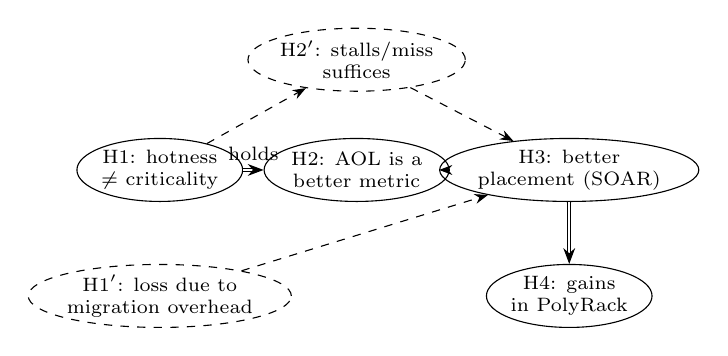
\begin{tikzpicture}[
  hyp/.style={ellipse, draw, align=center, font=\scriptsize,
              inner sep=0pt, minimum height=0.8cm},
  alt/.style={hyp, dashed},
  >={Stealth}]
  \node[hyp] (h1)  at (0,0.4)   {H1: hotness\\$\neq$ criticality};
  \node[alt] (h1a) at (0,-1.2)  {H1$'$: loss due to\\migration overhead};
  \node[hyp] (h2)  at (2.5,0.4) {H2: AOL is a\\better metric};
  \node[alt] (h2a) at (2.5,1.8) {H2$'$: stalls/miss\\suffices};
  \node[hyp] (h3)  at (5.2,0.4) {H3: better\\placement (SOAR)};
  \node[hyp] (h4)  at (5.2,-1.2) {H4: gains\\in PolyRack};
  \draw[->, double] (h1) -- node[above, font=\scriptsize]{holds} (h2);
  \draw[->, dashed] (h1) -- (h2a);
  \draw[->] (h2) -- (h3);
  \draw[->, dashed] (h2a) -- (h3);
  \draw[->, dashed] (h1a) -- (h3);
  \draw[->, double] (h3) -- (h4);
\end{tikzpicture}
\caption{Hypothesis tree. Solid: main hypotheses from~\cite{liu2025tiered};
dashed: alternatives we test in parallel. If H1$'$ holds instead of H1, the
problem is migration overhead: we skip Q2 and evaluate SOAR directly, since it
avoids most migrations.}
\label{fig:tree}
\end{figure}

\subsection{Q1: Are hotness metrics really informative?}
\begin{itemize}
  \item \textbf{Insight (I1):} out-of-order cores overlap independent misses,
        so high-MLP (often hot) accesses hide most of the slow-tier latency,
        while low-MLP accesses pay all of it.
  \item \textbf{Hypothesis (H1):} with the same DRAM capacity, placing the
        hot, high-MLP data in DRAM yields a \emph{higher} slowdown than
        placing the cold, low-MLP data in DRAM.
  \item \textbf{Refuted if:} on the microbenchmark, Hot-on-DRAM has a slowdown
        lower than or equal to Cold-on-DRAM.
  \item \textbf{Test (E1):} reproduce the hot/cold microbenchmark
        (sequential vs.\ pointer-chasing threads, cf.\
        Fig.~1 of~\cite{liu2025tiered}) with \emph{static} placements
        (All-on-DRAM, Hot-on-DRAM, Cold-on-DRAM) and migrations disabled, so
        that the result depends only on placement and not on migration cost.
  \item \textbf{Alternative (H1$'$):} SOTA systems lose because of the cost
        of their migrations, not because they mis-place data. \emph{Test
        (E1$'$):} run NoTier and the SOTA systems on the same benchmark and
        record the number of migrated pages. If the static placements perform
        alike but SOTA is slower than NoTier, H1$'$ holds.
\end{itemize}

\subsection{Q2: If not, how can a better metric be defined?}
\begin{itemize}
  \item \textbf{Insight (I2):} the average stall cycles per LLC miss vary by
        up to 4$\times$ across workloads~\cite{liu2025tiered}: MLP amortizes
        the latency, so a predictor that ignores it (LLC stalls/cycle, $P$)
        overestimates the slowdown of high-MLP workloads.
  \item \textbf{Hypothesis (H2):} the AOL-corrected predictor $P\times K$,
        with $K = f(\text{AOL})$ fitted empirically on our machine, correlates
        better with the measured slowdown than $P$ alone and than hotness
        (sampled access counts).
  \item \textbf{Refuted if:} the Pearson coefficient of $P\times K$ is not
        higher than that of $P$ (or of hotness) on our set of workloads.
  \item \textbf{Test (E2):} for each workload, measure the slowdown on the
        slow tier together with the counters for $P$, AOL and access counts;
        calibrate $a,b$ of $K$ with the sequential/pointer-chasing
        microbenchmarks; compare the Pearson coefficients of the three
        predictors (cf.\ Fig.~2 of~\cite{liu2025tiered}).
  \item \textbf{Alternative (H2$'$):} a simpler MLP-aware metric, the
        average LLC stalls per LLC miss without a fitted $K$, predicts the
        slowdown as well as $P\times K$. It is evaluated in the same
        experiment as E2 at no additional cost.
\end{itemize}

\subsection{Q3: With this metric, can we improve first data placement (SOAR)?}
\begin{itemize}
  \item \textbf{Insight (I3):} if the metric identifies performance-critical
        objects, placing them in DRAM at allocation time avoids both
        mis-placement and later migrations.
  \item \textbf{Hypothesis (H3):} SOAR achieves a lower slowdown than NoTier
        and every SOTA system at the same fast-tier capacity.
  \item \textbf{Refuted if:} NoTier or a SOTA system has an equal or lower
        slowdown (beyond run-to-run variance) in the majority of the
        (workload, slow-tier ratio) configurations.
  \item \textbf{Test (E3):} compare the slowdown of SOAR vs.\ NoTier, TPP,
        NBT, Nomad and Colloid on the selected workloads, at 10--90\%
        slow-tier ratios (cf.\ Fig.~4 and Table~4 of~\cite{liu2025tiered}).
\end{itemize}

\subsection{Q4: Can these elements improve PolyRack?}
\begin{itemize}
  \item \textbf{Insight (I4):} PolyRack disaggregates memory into dedicated
        memory servers reached through a CXL-class fabric, which creates a
        fast/slow memory hierarchy similar to a tiered server.
  \item \textbf{Hypothesis (H4):} AOL-based placement (SOAR) reduces the
        slowdown on PolyRack with respect to its default memory management.
  \item \textbf{Refuted if:} no reduction beyond run-to-run variance, after
        recalibrating $K$ for PolyRack.
  \item \textbf{Test (E4):} run the same workloads on PolyRack with and
        without SOAR, and compare against the traditional tiered server.
        Tested only if H3 holds.
\end{itemize}

\subsection{Handling failed hypotheses}
A refuted hypothesis is an anomaly that we analyze before moving on:
\begin{itemize}
  \item \emph{H1 fails:} our slow tier may hide latency differently (e.g.,
        lower latency ratio, more effective prefetching). We sweep the
        slow-tier latency (uncore frequency) to find whether the effect
        appears; if H1$'$ holds instead, we skip Q2 and evaluate SOAR
        directly, since it avoids most migrations.
  \item \emph{H2 fails:} we check whether $K$ fitted on our hardware has the
        same shape as in the paper, and use H2$'$ (if it holds) as the metric
        driving SOAR.
  \item \emph{H3 fails:} we analyze per workload which objects SOAR ranks
        incorrectly, and test whether recalibrating $K$ for our platform
        fixes the gap.
\end{itemize}

% =====================================================================
\section{Evaluation Methodology}
\label{sec:evaluation}

\subsection{Experimental setup}
We will first reproduce the results on a traditional server, and only then
move to PolyRack. Following~\cite{liu2025tiered}, if no real CXL device is
available the slow tier will be emulated with a remote NUMA node (lowering its
uncore frequency and disabling its cores, which in the paper yields 90/190\,ns
fast/slow latencies). We will use the open-source implementation of SOAR
(\url{https://github.com/MoatLab/SoarAlto}), Linux \texttt{perf} and the
offcore/LLC performance counters needed to compute $P$ and AOL, and
\texttt{numactl}/cgroups to control the fast/slow-tier ratio.
\todo{Confirm server access, CPU/kernel version, CXL vs.\ NUMA emulation, and
whether experiments run on bare metal or in a VM.}

\subsection{Workloads}
We will start from \texttt{bc-urand} and other graph workloads from the GAP
Benchmark Suite (GAPBS), which stress tiered memory with irregular accesses,
plus the hot/cold microbenchmark of Q1. Time permitting, we will add workloads
from the other categories used in the paper (machine learning, caching, HPC).
\todo{Agree on the final workload list with the TA (and on PolyRack's home
workloads).}

\subsection{Baselines and metrics}
Baselines: All-on-DRAM (upper bound), NoTier (first-touch, no migrations),
and the hotness-based SOTA systems TPP, NBT, Nomad and Colloid.
Metrics: slowdown relative to All-on-DRAM (lower is better), Pearson
correlation between predicted and measured slowdown, AOL and average memory
latency, and migration traffic (number of page promotions/demotions), all
measured across several fast/slow-tier ratios (e.g., 10--90\% of the
workload's RSS in the slow tier). Every configuration is run at least three
times; we report mean and standard deviation, and consider two policies
different only when their means differ by more than the run-to-run standard
deviation.

% =====================================================================
\section{Final Deliverable}
\label{sec:deliverable}

\subsection{Concrete goals}
By the end of the semester we want to (1) have a working tiered-memory setup
with the baselines and SOAR running, (2) confirm or refute H1--H3 (and the
alternatives H1$'$, H2$'$) on our hardware, and (3) if time permits, provide a
first evaluation of H4 on PolyRack.

\subsection{Expected results}
Our key figure (Fig.~\ref{fig:expected}) will plot the slowdown w.r.t.\
All-on-DRAM (Y-axis) as a function of the fraction of the working set placed
in the slow tier (X-axis), for NoTier, a hotness-based SOTA system and SOAR.
We expect slowdown to grow with the slow-tier ratio for all policies, with
SOTA sometimes worse than NoTier (due to useless migrations) and SOAR
consistently below both. We will also show the
predicted-vs.-measured slowdown scatter plot for $P$, $P\times K$, hotness
and stalls/miss (Q2).

\begin{figure}[t]
\centering
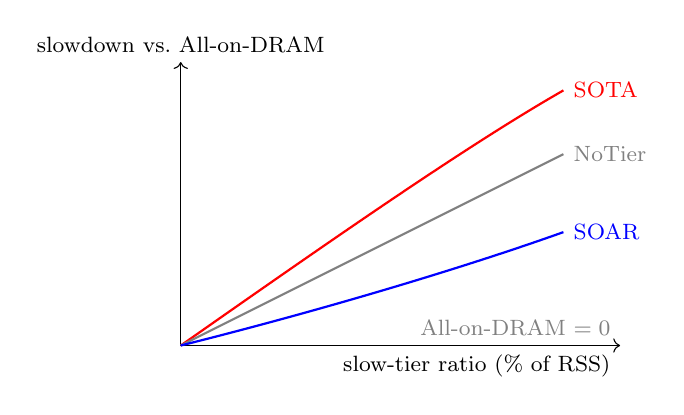
\begin{tikzpicture}[scale=0.9, font=\footnotesize]
  \draw[->] (0,0) -- (6.2,0) node[below left, align=right]
    {slow-tier ratio (\% of RSS)};
  \draw[->] (0,0) -- (0,4) node[above, align=center]
    {slowdown vs.\ All-on-DRAM};
  \draw[thick, red]    (0,0) .. controls (2,1.4) and (4,2.8) .. (5.4,3.6)
    node[right] {SOTA};
  \draw[thick, gray]   (0,0) .. controls (2,1.0) and (4,2.0) .. (5.4,2.7)
    node[right] {NoTier};
  \draw[thick, blue]   (0,0) .. controls (2,0.5) and (4,1.1) .. (5.4,1.6)
    node[right] {SOAR};
  \node[gray, above left] at (6.2,0) {All-on-DRAM $=0$};
\end{tikzpicture}
\caption{Sketch of the expected main result. All-on-DRAM is the zero line;
NoTier is first-touch without migrations. AOL-based placement (SOAR) keeps the
slowdown lower than hotness-based SOTA and NoTier across slow-tier ratios.}
\label{fig:expected}
\end{figure}

% =====================================================================
\section{Plan and Milestones}
\label{sec:milestones}
Each milestone lists its deadline and the follow-up question it answers.
\begin{enumerate}
  \item \textbf{Oct.~13:} proposal and presentation.
        \emph{Follow-up:} which servers, CXL device or NUMA emulation, and
        workloads are available to us (Sec.~\ref{sec:open})?
  \item \textbf{Oct.~23:} environment ready: tiered (or NUMA-emulated)
        memory, SOAR code and baselines built, counters for $P$ and AOL
        readable with \texttt{perf}.
        \emph{Follow-up:} does our CPU expose the offcore counters AOL needs?
  \item \textbf{Oct.~30:} E1 and E1$'$ done.
        \emph{Follow-up:} does H1 hold on our hardware, or H1$'$?
  \item \textbf{Nov.~12 (status report):} E2 done ($K$ calibrated, Pearson
        coefficients of $P$, $P\times K$, hotness and H2$'$); first SOAR
        results on \texttt{bc-urand}.
        \emph{Follow-up:} which metric should drive SOAR on our platform?
  \item \textbf{Nov.~27:} E3 done on all selected workloads and slow-tier
        ratios.
        \emph{Follow-up:} on which configurations does SOAR lose, and why?
  \item \textbf{Dec.~4:} (if time permits) E4 on PolyRack.
        \emph{Follow-up:} can AOL be measured and calibrated on PolyRack's
        memory path?
  \item \textbf{Dec.~10 / Dec.~17 / Dec.~20:} poster, poster session and
        final report.
\end{enumerate}

% =====================================================================
\section{Open Questions for the Teaching Team}
\label{sec:open}
\begin{enumerate}
  \item Will we test AOL/SOAR directly on PolyRack, or on a traditional
        server beforehand? (Our plan assumes the latter.)
  \item Which home workloads will we work with?
  \item How does access to the servers work?
  \item How will we set up our experiments (programming language, bare metal
        vs.\ VM, etc.)?
\end{enumerate}

% =====================================================================
\begin{thebibliography}{9}
\bibitem{liu2025tiered}
J.~Liu, H.~Hadian, H.~Xu, and H.~Li, ``Tiered Memory Management Beyond
Hotness,'' in \emph{19th USENIX Symposium on Operating Systems Design and
Implementation (OSDI)}, Boston, MA, USA, Jul. 2025.

\bibitem{polyrack}
P.~Poorsarvi Tehrani, S.~Lin, A.~Ning, B.~Falsafi, D.~Atienza, T.~Bourgeat,
and S.~Kashyap, ``PolyRack: Servers for the Post-Moore Era,'' EPFL, 2026.
\end{thebibliography}

\end{document}
